\documentclass[]{exam}

\usepackage{amsmath}
\usepackage{amssymb}
\usepackage{tikz}
\usepackage{tabularx}
\tikzstyle{vertex}=[circle,fill=black!25,minimum size=17pt,inner sep=0pt]

\pagestyle{empty}
\extrawidth{.5in}

\def\bonuson{\renewcommand\partlabel{*(\thepartno)}}
\def\bonusoff{\renewcommand\partlabel{(\thepartno)}}

\begin{document}
  \begin{center}
    \fbox{\fbox{\parbox{5.5in}{\centering Answer the questions in the spaces
    provided on the question sheets. If you run out of room for an answer,
    continue on a separate sheet of paper.}}}
  \end{center}

  \begin{questions}
    \question Define the directed graph $G$ as follows:

      \bigskip

      \begin{center}
        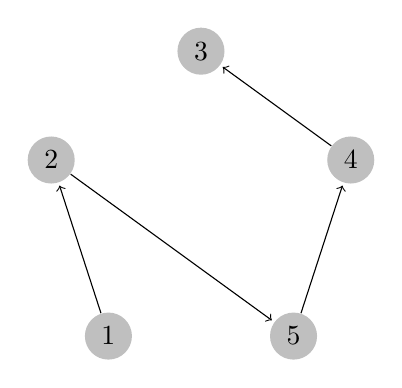
\begin{tikzpicture}[shorten >=1pt,->]
          \foreach \name/\angle/\text in {P-1/234/1, P-2/162/2, 
                                          P-3/90/3, P-4/18/4, P-5/-54/5}
            \node[vertex,xshift=6cm,yshift=.5cm] (\name) at (\angle:2cm) {$\text$};
          \foreach \from/\to in {1/2,2/5,5/4,4/3}
            \draw (P-\from) -- (P-\to);
        \end{tikzpicture}
      \end{center}

      \bigskip

      \begin{parts}
        \part Find $G^2$.
          \begin{solution}~\\
            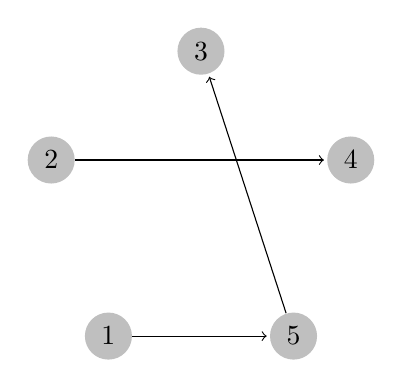
\begin{tikzpicture}[shorten >=1pt,->]
              \foreach \name/\angle/\text in {P-1/234/1, P-2/162/2, 
                                              P-3/90/3, P-4/18/4, P-5/-54/5}
                \node[vertex,xshift=6cm,yshift=.5cm] (\name) at (\angle:2cm) {$\text$};
              \foreach \from/\to in {1/5,2/4,5/3}
                \draw (P-\from) -- (P-\to);
            \end{tikzpicture}
          \end{solution}
          \vspace{\stretch{1}}

        \part Find $G^+$.
          \begin{solution}~\\
            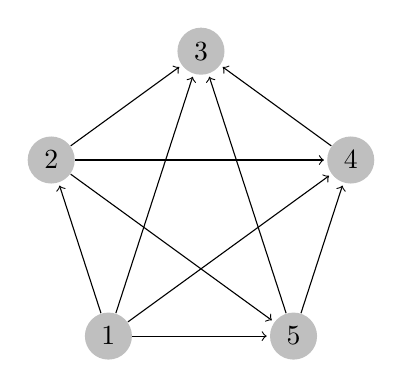
\begin{tikzpicture}[shorten >=1pt,->]
              \foreach \name/\angle/\text in {P-1/234/1, P-2/162/2, 
                                              P-3/90/3, P-4/18/4, P-5/-54/5}
                \node[vertex,xshift=6cm,yshift=.5cm] (\name) at (\angle:2cm) {$\text$};
              \foreach \from/\to in {1/2,2/5,5/4,4/3,1/5,2/4,5/3,1/4,2/3,1/3}
                \draw (P-\from) -- (P-\to);
            \end{tikzpicture}
          \end{solution}
          \vspace{\stretch{1}}
      \end{parts}

    \newpage

    \question Define the directed graph $G$ as follows:

      \bigskip

      \begin{center}
        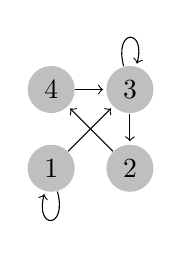
\begin{tikzpicture}[shorten >=1pt,->]
          \node[vertex] (1) at (0,0) {1};
          \node[vertex,right of=1] (2) {2};
          \node[vertex,above of=2] (3) {3};
          \node[vertex,above of=1] (4) {4};
          \path
            (1) edge[loop below] (1)
            (3) edge[loop above] (3)
            (1) edge (3)
            (3) edge (2)
            (2) edge (4)
            (4) edge (3);
        \end{tikzpicture}
      \end{center}

      \bigskip

      \begin{parts}
        \part Complete the \emph{adjacency matrix}, $A$, for $G$.

          \bigskip

          \ifprintanswers
            \vspace{-\baselineskip}
            \begin{solution}~\\[1\baselineskip]
              {$\begin{bmatrix}
                1 & 0 & 1 & 0 \\
                0 & 0 & 0 & 1 \\
                0 & 1 & 1 & 0 \\
                0 & 0 & 1 & 0
              \end{bmatrix}$}
            \end{solution}
          \else
            $\begin{bmatrix}
              \hspace{20em}\vspace{18em}
            \end{bmatrix}$
          \fi

        \bigskip
        \bigskip

        \part Compute $A^2$.

          \bigskip

          \ifprintanswers
            \vspace{-\baselineskip}
            \begin{solution}~\\[1\baselineskip]
              {$\begin{bmatrix}
                1 & 1 & 1 & 0 \\
                0 & 0 & 1 & 0 \\
                0 & 1 & 1 & 1 \\
                0 & 1 & 1 & 0
              \end{bmatrix}$}
            \end{solution}
          \else
            $\begin{bmatrix}
              \hspace{20em}\vspace{18em}
            \end{bmatrix}$
          \fi
      \end{parts}
  \end{questions}
\end{document}
